\chapter[Catchup]{Catchup}

\section[2026/03/26]{Thursday, 26 March 2026}
\label{sec:20260326}

This chapter covers everything that has changed since the last proper labbook entry. I've been bad about keeping up with this so this is a big dump of what happened, what worked, and what didn't.


\subsection{Dataset Generator Refactor}

The old code had separate files for everything --- \texttt{virtual\_dataloader.py}, \texttt{virtual\_dataset.py}, \texttt{virtual\_preprocessor.py} as well as \texttt{dataloader.py}, \texttt{dataset.py}, \texttt{preprocessor.py}, \texttt{depth\_estimation.py}. The architecture has been updated to use a unified pipeline:

\begin{verbatim}
COCO data          Virtual data
    |                   |
coco_adapter.py    virtual_adapter.py
         |         |
        dataset.py          <-- single Dataset class
             |
        preprocessor.py     <-- single graph builder
             |
        dataloader.py       <-- single DataLoader
\end{verbatim}

Two reasons for this:
\begin{compactitem}
  \item After the adapter it doesn't matter where the data came from, the rest of the pipeline is identical
  \item Can train on synthetic data first then swap to COCO without changing anything downstream
\end{compactitem}


\subsubsection{Extractor changes}

Keypoint format changed from $[x,y,v]$ to $[x,y,z,v]$ per joint (51 $\to$ 68 values per person). Per-joint depth is strictly better than one depth value per person. $z$ is world-space Euclidean distance from camera to joint in metres --- consistent across all camera positions, matches MiDaS semantics after normalisation.

Visibility changed from $0/2$ to $0/1/2$ with raycast occlusion detection. Occluded joints are real training signal --- marking them as invisible was losing information.

\texttt{calculate\_distance\_to\_camera} was removed --- redundant now that there is per-joint $z$.

Out-of-frame joints position changed from $[0.0, 0.0]$ to $[-1.0, -1.0]$. Zero is a real pixel location (top-left corner), $-1$ is an unambiguous sentinel meaning ``no valid position''. The GAT uses visibility $v=0$ to ignore these joints during message passing but the position itself should also signal invalidity explicitly.


\subsubsection{Renderer changes}

Filenames changed to \texttt{<guid>\_<n>.png} / \texttt{<guid>\_<n>.json}. GUIDs eliminate ID collisions, the \texttt{\_n} suffix allows filtering by person count without parsing JSON. \texttt{num\_people} was added to image metadata for debugging and dataset statistics.


\subsubsection{Virtual adapter}

Loads a folder of \texttt{<guid>\_n.png/<guid>\_n.json} pairs and scans the folder to filter using min and max people. Converts from the per-image JSON (68 floats per person) to the unified output:

\begin{verbatim}
{
    "image":      tensor [3, H, W],
    "keypoints":  list of tensor [17, 4],  # [x, y, z, v]
    "img_id":     str,
    "num_people": int
}
\end{verbatim}

No transforms, no normalisation, no MiDaS --- just reading and reshaping. Everything else happens downstream.


\subsubsection{COCO adapter}

Loads COCO 2017 person keypoint annotations via pycocotools, filters by min/max person count the same way as the virtual adapter. MiDaS DPT\_Hybrid is initialised once at construction time and used to estimate a depth map per image. Depth is then sampled at each keypoint's pixel location.

Converts from COCO's flat format (51 floats per person, COCO visibility 0/1/2) to the same unified output as the virtual adapter.

Visibility is handled explicitly:

\begin{center}
\begin{tabular}{lll}
\toprule
COCO $v$ & Position & Depth \\
\midrule
0 (not labelled) & $[-1, -1]$ & 0 \\
1 (occluded) & real $x, y$ & MiDaS sampled \\
2 (visible) & real $x, y$ & MiDaS sampled \\
\bottomrule
\end{tabular}
\end{center}


\subsubsection{Dataset}

Single shared Dataset class that sits between the adapters and the rest of the pipeline. Accepts either adapter and applies a consistent transform so everything downstream sees the same tensor shapes regardless of data source.

\begin{compactitem}
  \item Image resized to fit within \texttt{target\_size} $\times$ \texttt{target\_size} preserving aspect ratio
  \item Symmetrically padded to exactly \texttt{target\_size} $\times$ \texttt{target\_size}
  \item Keypoint $x, y$ scaled and shifted to match the new image dimensions
  \item $z$ and $v$ columns left untouched
  \item Joints with $v=0$ (sentinel $-1, -1$) are not transformed
\end{compactitem}


\subsubsection{Dataloader}

Wraps a PoseDataset with a custom collate function. Images stacked into a single tensor, keypoints kept as a list of lists since person count varies per image. \texttt{batch\_size} is an explicit argument controlled from \texttt{config.yaml}.


\subsubsection{Preprocessor}

Single unified graph builder. Converts a DataLoader batch into PyTorch Geometric graphs ready for the GAT. One graph per image, all people's joints are nodes in the same graph.

Joints with $v=0$ are excluded entirely --- no position, no node. Everything else becomes a node with features:

\begin{center}
\begin{tabular}{ll}
\toprule
Feature & Description \\
\midrule
$x_{\text{norm}}$ & $x$ normalised to $[0, 1]$ by image size \\
$y_{\text{norm}}$ & $y$ normalised to $[0, 1]$ by image size \\
$z_{\text{norm}}$ & depth normalised per-graph min-max over valid joints \\
$v_{\text{norm}}$ & visibility normalised ($0 \to 0.0$, $1 \to 0.5$, $2 \to 1.0$) \\
\bottomrule
\end{tabular}
\end{center}

Separate tensors per graph: \texttt{joint\_types} ($[N]$ long, index 0--16 for GAT embedding layer) and \texttt{person\_labels} ($[N]$ long, ground truth person assignment for training).

Edges are built using kNN with $k=8$ on $(x_{\text{norm}}, y_{\text{norm}}, z_{\text{norm}})$ --- depth is part of the proximity calculation so joints that are close in 3D get connected even if far apart in 2D.

Key decisions:
\begin{compactitem}
  \item Per-graph depth normalisation --- MiDaS and metric depth have different absolute scales, normalising per-graph makes both sources comparable
  \item \texttt{joint\_types} separate from features --- lets the GAT learn a per-joint-type embedding independently of position
  \item kNN includes depth --- richer connectivity than 2D-only
\end{compactitem}

All pipeline tests passed --- see \texttt{outputs/test\_outputs/data}.


% ────────────────────────────────────────────────────────────
\subsection{GAT}

The GAT (Graph Attention Network) takes the graph of joints built by the preprocessor and produces a 128-dimensional embedding for each joint. The goal is for joints belonging to the same person to end up close together in this 128D space, and joints from different people to be far apart.

The architecture:
\begin{compactitem}
  \item Each joint starts as a 4-value feature vector $[x, y, z, v]$ plus a learned 32-dim embedding for its joint type (nose, left knee, etc.)
  \item Two GATv2 layers with 4 attention heads do message passing --- each joint updates its representation by attending to its neighbours
  \item A final linear projection maps down to 128 dimensions
  \item L2 normalisation so all embeddings live on the unit hypersphere
\end{compactitem}

The joint type embedding matters --- a left knee should have different characteristics than a nose regardless of position, and keeping this separate from the spatial features lets the GAT learn that independently.


\subsubsection{Training (isolation phase)}

The GAT is trained in isolation using contrastive loss only. Pull same-person joint embeddings together, push different-person joint embeddings apart. No grouping head yet --- just verifying the embedding space is structured correctly before adding the next component.

Config:
\begin{verbatim}
gat:
  num_joint_types: 17
  joint_embedding_dim: 32
  raw_feature_dim: 4
  hidden_dim: 64
  output_dim: 128
  num_layers: 2
  num_heads: 4
  dropout: 0.1
  use_layer_norm: true
  l2_normalize: true

loss:
  contrastive_margin: 0.5
\end{verbatim}


\subsubsection{Isolation test results}

Four sanity checks passed:
\begin{compactitem}
  \item Forward pass --- output shape $[N, 128]$
  \item L2 normalisation --- all norms $\approx 1.0$
  \item Loss computation --- scalar, no NaN, $\geq 0$
  \item Gradient flow --- all parameters receive gradients
\end{compactitem}

Two separability runs on a fixed scene with 5 people and 85 joints:

\begin{center}
\begin{tabular}{lcccc}
\toprule
Metric & \multicolumn{2}{c}{100 steps / 8 graphs} & \multicolumn{2}{c}{500 steps / 16 graphs} \\
 & Before & After & Before & After \\
\midrule
Silhouette & $-0.043$ & $-0.082$ & $-0.030$ & $-0.042$ \\
Distance ratio & 1.006 & 1.108 & 0.992 & 1.020 \\
kNN accuracy & 0.630 & 0.983 & 0.596 & 0.985 \\
\bottomrule
\end{tabular}
\end{center}

kNN accuracy is the most meaningful number --- 0.983 and 0.985 means almost every joint's 5 nearest neighbours in embedding space belonged to the same person. The distance ratio is noticeably better in the 100-step run (1.108 vs 1.020) which is expected --- 16 graphs covers more diverse scenes making the task harder. Silhouette stays negative in both runs due to geometric compression on the unit hypersphere --- not a useful metric here, reported for completeness only.

\textbf{PCA} projects the 128D embeddings down to 2D by finding the axes of maximum variance. Before training both plots show colours scattered and mixed with PCA variance explained around 87\%. After 100 steps: five tight, clearly separated clusters with PCA variance explained at 99.17\%. After 500 steps: same clean result at 97.56\%.

\textbf{t-SNE} preserves local neighbourhood structure rather than global variance. Same-colour points clustering together in both after-training plots confirms the embedding space is well structured.

See \texttt{outputs/test\_outputs/gat}.


% ────────────────────────────────────────────────────────────
\subsection{Grouping Head Selection}

GAT isolation verified. The next step was the grouping head --- takes the embeddings from the GAT and produces the final joint-to-person assignment. Four candidates were considered:

\begin{compactitem}
  \item Deep Embedded Clustering (DEC)
  \item DETR (DEtection TRansformer)
  \item Graph partitioning
  \item Slot attention
\end{compactitem}


% ────────────────────────────────────────────────────────────
\subsection{DEC (Deep Embedded Clustering)}

DEC takes embeddings and learns $K$ cluster centres in the same embedding space. Each joint gets a soft assignment $q$ based on distance to each centre using a Student's $t$-distribution. A sharpened target distribution $p$ is computed from $q$ and the model is trained to minimise KL divergence between them --- pushing soft assignments toward harder, more confident ones over time.

Cluster centres are initialised with k-means++ before training. One important detail: $p$ is updated every \texttt{update\_interval} steps rather than every step. Updating every step causes cluster collapse --- the model chases a moving target and all joints pile into one cluster by step 150. Periodic updates let the centres stabilise between target refreshes.


\subsubsection{What I tried and why it kept failing}

\textbf{Attempt 1 --- random GAT embeddings.}
With an untrained GAT all joints are roughly equidistant from all cluster centres, so $q$ is nearly uniform across all $K$ clusters. $p$ is computed from $q$ so $p \approx q$, which means $\text{KL}(p \| q) \approx 0$ immediately --- no loss, no gradient, no learning.

\textbf{Attempt 2 --- pre-trained GAT embeddings.}
With 200 steps of GAT pre-training, k-means++ initialised perfectly (accuracy 1.0 before any DEC training). But then DEC actively degraded:

\begin{verbatim}
Before training: accuracy = 1.0000
Step  25: accuracy=1.0000  loss=0.0661
...
Step 125: accuracy=0.5765  loss=0.0005
Step 150: accuracy=0.2000  loss=0.0002
\end{verbatim}

This is cluster collapse --- $p$ was being recomputed from $q$ every step, the model chased a moving target, and all joints piled into one cluster. Fixed with periodic $p$ updates but a deeper problem remained: if the GAT is good there's nothing for DEC to do.

\textbf{Attempt 3 --- periodic updates, real scale (17 joints per person, 128D).}
Switched to fabricated embeddings (Gaussian blobs on the unit hypersphere with known ground truth) to control difficulty. Hit a hard ceiling:

\begin{verbatim}
Step 250: accuracy=0.7647  loss=0.0273
Step 300: accuracy=0.7647  loss=0.0272
...
Step 1000: accuracy=0.7647  loss=0.0274
\end{verbatim}

0.7647 exactly --- 4 out of 5 clusters correct, one pair always confused regardless of noise level or number of steps. This is the curse of dimensionality --- 17 points in 128D is too sparse for the Student's $t$ soft assignments to produce a meaningful gradient.

\textbf{Attempt 4 --- 50 joints per person.}
Bumped \texttt{n\_per\_person} to 50:

\begin{verbatim}
Before training: accuracy = 0.6200
Step 250: accuracy=0.9680
Step 300: accuracy=1.0000
\end{verbatim}

DEC works --- but only with 3$\times$ more points per cluster than the real problem has.


\subsubsection{Isolation test results}

5 clusters, 50 points per cluster, 128D, \texttt{update\_interval=20}:

\begin{center}
\begin{tabular}{lcc}
\toprule
 & Before training & After training \\
\midrule
Easy (noise=0.05) & 1.000 & 1.000 \\
Medium (noise=0.1) & 0.620 & 1.000 \\
\bottomrule
\end{tabular}
\end{center}

Accuracy measured with Hungarian matching since DEC cluster indices are arbitrary.


\subsubsection{Why DEC isn't the right head}

DEC is fully unsupervised --- it never sees ground truth labels. It can only sharpen assignments that are already roughly correct, it has no signal to fix wrong ones. With 17 joints per person in 128D there is a hard ceiling at 0.8 regardless of tuning. If the GAT is doing its job, kNN accuracy on the embeddings is already 0.98--1.0 and k-means++ alone at inference time would give near-perfect assignments. DEC adds complexity and collapse risk without improving on the initialisation.

The right grouping head needs to learn from ground truth labels. Graph partitioning and slot attention both do this.


% ────────────────────────────────────────────────────────────
\subsection{Slot Attention}

\subsubsection{Why slot attention}

DEC failed at realistic scale because it is unsupervised. Slot attention is trained end-to-end with ground truth person assignments via Hungarian-matched cross entropy.

\subsubsection{What it does}

Slot attention is an iterative competitive attention mechanism. $K$ slot vectors are initialised by sampling from a learned Gaussian distribution, one slot per person. Over several iterations each slot attends to all joints and competes for the ones it best represents. The competition is enforced by applying softmax over slots rather than over joints --- each joint's attention weights sum to 1 across all slots, so if two slots compete for the same joint the better-matching one wins.

After iterative refinement the final slot vectors score each joint via dot product, producing logits $[N, K]$. Hungarian matching finds the optimal bijection between predicted slots and ground truth people, and cross entropy is computed on the matched assignments.

The architecture:
\begin{verbatim}
Inputs:  embeddings [N, D]  L2-normalised GAT embeddings
         k          int     number of people in this scene

Slots sampled from learned mu, sigma  ->  [K, D]

For num_iterations:
    norm(slots)   ->  queries  [K, D]
    norm(inputs)  ->  keys     [N, D]
                      values   [N, D]

    scores   =  queries . keys^T * scale     [K, N]
    softmax over slots  (competition)        [K, N]
    normalise within each slot               [K, N]
    updates  =  weighted sum of values       [K, D]
    slots    =  GRU(updates, slots)          [K, D]
    slots    =  slots + FF(LayerNorm(slots)) [K, D]

slot_keys  =  linear(slots)                 [K, D]
logits     =  embeddings . slot_keys^T      [N, K]
\end{verbatim}

Loss: Hungarian matching between predicted slots and ground truth people, then cross entropy on matched assignments.

Config:
\begin{verbatim}
slot_attention:
  num_iterations: 7
  slot_weight:    1.0
\end{verbatim}


\subsubsection{What went wrong during testing}

\textbf{Instability at lr=$10^{-3}$, 3 iterations} --- the model found the correct solution early (accuracy 1.0 at step 100) but then overshot and lost it, ending at 0.78. Slots reinitialise from the learned Gaussian every forward pass --- with only 3 iterations they do not always converge, producing noisy gradient signal.

\textbf{Fix 1 --- more iterations.} Increasing \texttt{num\_iterations} from 3 to 7 stabilised the assignments within each forward pass and produced cleaner gradient signal.

\textbf{Fix 2 --- cosine LR schedule.} A flat lr of $10^{-3}$ caused overshooting. A cosine schedule decaying from $10^{-3}$ to $10^{-5}$ allows fast early learning and fine-grained settling.


\subsubsection{Isolation test results}

5 clusters, 17 joints per person (real scale), 128D, 500 steps, cosine LR $10^{-3} \to 10^{-5}$:

\begin{center}
\begin{tabular}{lccc}
\toprule
 & Before training & Best accuracy & Step reached \\
\midrule
Easy (noise=0.05) & 0.459 & 1.000 & 250 \\
Hard (noise=0.15) & 0.400 & 1.000 & 200 \\
\bottomrule
\end{tabular}
\end{center}

Both tests reach perfect accuracy at realistic joint counts --- 17 joints per person, the same scale the real problem provides. DEC hit a hard ceiling of 0.8 at this scale and never improved.


% ────────────────────────────────────────────────────────────
\subsection{Graph Partitioning}

\subsubsection{What it does}

Graph partitioning frames the grouping problem as binary edge classification. For every pair of joints $(i, j)$ the model predicts whether they belong to the same person. After thresholding, connected components on the resulting affinity graph recover the person groups without any explicit knowledge of $K$.

This is a fundamentally different framing from slot attention. Slot attention assigns joints to $K$ pre-specified slots via competitive attention. Graph partitioning makes pairwise same/different decisions and lets the group structure emerge from the graph topology. $K$ does not need to be specified at inference time --- it falls out naturally from the number of connected components.

For each pair $(i, j)$ the feature vector is:
\begin{equation}
f(i, j) = [e_i - e_j \; \| \; e_i \odot e_j] \in \mathbb{R}^{2D}
\end{equation}
where $e_i, e_j$ are L2-normalised GAT embeddings. The difference captures direction between the two points in embedding space; the element-wise product captures co-activation. The MLP maps $\mathbb{R}^{2D}$ to a scalar logit per pair.

Groups are recovered at inference by thresholding predicted affinities at 0.5 and finding connected components via union-find.

Loss is binary cross entropy over all $N(N-1)/2$ pairs. With 5 people $\times$ 17 joints there are 680 same-person pairs and 2890 different-person pairs --- a 4:1 class imbalance. \texttt{pos\_weight = n\_neg / n\_pos} (clamped at 10) upscales the positive class.

Two metrics tracked:
\begin{compactitem}
  \item \textbf{Edge F1} --- precision/recall balance on the binary pair classification (accuracy is misleading under class imbalance)
  \item \textbf{Grouping accuracy} --- end-to-end metric: thresholded edges $\to$ connected components $\to$ Hungarian matching against ground truth
\end{compactitem}


\subsubsection{Isolation test results}

5 clusters, 17 joints per person (real scale), 128D, 500 steps, cosine LR $10^{-3} \to 10^{-5}$:

\begin{center}
\begin{tabular}{lcccc}
\toprule
 & Before training & Best F1 & Best grouping acc & Step \\
\midrule
Easy (noise=0.05) & F1=0.083 / acc=0.212 & 1.000 & 1.000 & 50 \\
Hard (noise=0.15) & F1=0.235 / acc=0.200 & 1.000 & 1.000 & 50 \\
\bottomrule
\end{tabular}
\end{center}

Perfect F1 and grouping accuracy by step 50 on both tests, holding stable for the remaining 450 steps with loss decaying smoothly to near zero. The cleanest result of all three grouping heads tested.


\subsubsection{Comparison across all grouping heads}

\begin{center}
\begin{tabular}{lcccc}
\toprule
 & DEC & Slot attention & Graph partitioning \\
\midrule
Supervision & Unsupervised & Supervised (CE) & Supervised (BCE) \\
Ceiling at 17 joints / 128D & 0.8 & 1.0 & 1.0 \\
Requires $K$ at inference & Yes & Yes & No \\
Stability & Collapsed & Noisy & Very stable \\
Steps to converge & Never & $\sim$200 & $\sim$50 \\
End-to-end trainable & Weakly & Yes & Yes \\
\bottomrule
\end{tabular}
\end{center}

The key practical advantage of graph partitioning is stability and convergence speed --- direct binary supervision from 3570 labelled pairs per scene is dense and unambiguous. The key theoretical advantage over slot attention is that $K$ does not need to be known at inference time.


% ────────────────────────────────────────────────────────────
\subsection{DETR --- Rationale for Exclusion}

DETR was considered as a fourth grouping head but not pursued to isolation testing.

\textbf{Architectural overlap with slot attention.} DETR's decoder is a superset of slot attention --- it adds self-attention between queries and a heavier feed-forward stack, but the core mechanism is the same iterative cross-attention competition. The additional complexity adds no meaningful capability for this problem.

\textbf{The null object problem.} DETR handles variable detection counts by padding predictions with a learned ``no object'' class. Resolving the null value instability encountered in the preliminary implementation requires careful loss masking and balanced sampling --- engineering overhead with no benefit for this problem where the number of people per scene is bounded and known at training time.

\textbf{The comparison is already complete without it.} The four approaches evaluated (kNN on GAT embeddings, DEC, slot attention, graph partitioning) span the relevant design space: unsupervised vs supervised, slot-based vs pairwise, $K$-required vs $K$-free. DETR would not add a meaningfully distinct data point.


% ────────────────────────────────────────────────────────────
\subsection{Experimental Results}

\subsubsection{Metrics}

\textbf{PGA (Pose Grouping Accuracy).} The primary metric. For each scene, predicted person groups are matched to ground truth people via Hungarian matching --- finding the optimal bijection between predicted and ground truth labels. PGA is the fraction of joints assigned to the correct person under this optimal matching. A score of 1.0 means every joint was grouped correctly. This metric is permutation-invariant.

\textbf{NMI (Normalised Mutual Information).} Measures the quality of the GAT embeddings independently of the grouping head. K-means is run on the embeddings with ground truth $K$, and NMI measures how much information the resulting clusters share with the ground truth person labels. NMI is the same across all methods evaluated from the same checkpoint because it depends only on the embeddings, not the grouping head.

\textbf{ARI (Adjusted Rand Index).} A second embedding quality metric. Measures agreement between k-means clustering and ground truth, corrected for chance. Like NMI, it is the same across all heads from the same checkpoint.

\textbf{Detection F1.} Measures whether the method correctly counts the number of people in the scene. For kNN this is always 1.0 because ground truth $K$ is provided. For slot attention $K$ is also provided. For graph partitioning $K$ is inferred from connected components --- if the edge threshold splits or merges groups, F1 drops.

\textbf{Per-joint accuracy.} PGA broken down by COCO joint type. Reveals whether certain joints are harder to group correctly --- typically extremities (ankles, wrists) which are more likely to be occluded or close to another person's joints.


\subsubsection{Experiment 1 --- Synthetic test set}

All models trained on 400 virtual scenes (100 each at 2/3/4/5 people), evaluated on 100 held-out virtual scenes. Training: 50 epochs, cosine LR $10^{-3} \to 10^{-5}$, AdamW.

\begin{center}
\begin{tabular}{lccccc}
\toprule
Method & PGA & Std & NMI & ARI & Det F1 \\
\midrule
kNN (contrastive GAT) & 0.994 & 0.012 & 0.987 & 0.987 & 1.000 \\
kNN (partition GAT) & 0.995 & 0.012 & 0.987 & 0.987 & 1.000 \\
Graph partitioning & 0.954 & 0.115 & 0.987 & 0.987 & 0.973 \\
kNN (slot GAT) & 0.994 & 0.015 & 0.988 & 0.987 & 1.000 \\
Slot attention & 0.858 & 0.143 & 0.988 & 0.987 & 0.935 \\
\bottomrule
\end{tabular}
\end{center}

Per-joint accuracy on synthetic data:

\begin{center}
\small
\begin{tabular}{lccc}
\toprule
Joint & kNN & Graph partition & Slot attention \\
\midrule
nose & 1.000 & 0.955 & 0.852 \\
left eye & 1.000 & 0.955 & 0.852 \\
right eye & 1.000 & 0.955 & 0.854 \\
left ear & 1.000 & 0.955 & 0.854 \\
right ear & 1.000 & 0.955 & 0.856 \\
left shoulder & 1.000 & 0.955 & 0.861 \\
right shoulder & 1.000 & 0.955 & 0.864 \\
left elbow & 0.992 & 0.955 & 0.860 \\
right elbow & 0.984 & 0.947 & 0.852 \\
left wrist & 0.994 & 0.955 & 0.873 \\
right wrist & 0.975 & 0.952 & 0.853 \\
left hip & 1.000 & 0.955 & 0.863 \\
right hip & 1.000 & 0.955 & 0.863 \\
left knee & 1.000 & 0.955 & 0.868 \\
right knee & 0.996 & 0.953 & 0.864 \\
left ankle & 0.990 & 0.955 & 0.855 \\
right ankle & 0.984 & 0.941 & 0.842 \\
\bottomrule
\end{tabular}
\end{center}

On synthetic data kNN is the strongest method. The GAT with contrastive loss produces near-perfect embeddings (NMI 0.987, ARI 0.987) and k-means is sufficient to recover the correct groups. The learned grouping heads do not improve on this. The head loss going to near zero by epoch 36 for graph partitioning confirms that the edge classifier solved its task quickly and stopped contributing meaningful gradient signal --- the GAT was already making the problem trivially easy.


\subsubsection{Experiment 2 --- COCO val2017 (zero-shot transfer)}

The same trained checkpoints evaluated on COCO val2017 with no fine-tuning. MiDaS DPT\_Hybrid provides per-joint depth estimates. 2346 images, all with at least one annotated person. This is a zero-shot sim-to-real transfer test --- the models have never seen real images during training.

\begin{center}
\begin{tabular}{lccccc}
\toprule
Method & PGA & Std & NMI & ARI & Det F1 \\
\midrule
kNN (contrastive GAT) & \textbf{0.838} & 0.194 & 0.754 & 0.692 & 1.000 \\
kNN (partition GAT) & 0.836 & 0.195 & 0.751 & 0.687 & 1.000 \\
kNN (slot GAT) & 0.828 & 0.202 & 0.740 & 0.675 & 1.000 \\
Slot attention & 0.788 & 0.236 & 0.740 & 0.675 & 0.920 \\
Graph partitioning & 0.752 & 0.266 & 0.751 & 0.687 & 0.802 \\
\bottomrule
\end{tabular}
\end{center}

Per-joint accuracy on COCO:

\begin{center}
\small
\begin{tabular}{lccc}
\toprule
Joint & kNN & Graph partition & Slot attention \\
\midrule
nose & 0.832 & 0.748 & 0.786 \\
left eye & 0.818 & 0.733 & 0.778 \\
right eye & 0.819 & 0.741 & 0.779 \\
left ear & 0.796 & 0.697 & 0.744 \\
right ear & 0.807 & 0.709 & 0.761 \\
left shoulder & 0.835 & 0.746 & 0.780 \\
right shoulder & 0.838 & 0.747 & 0.786 \\
left elbow & 0.841 & 0.739 & 0.780 \\
right elbow & 0.833 & 0.748 & 0.783 \\
left wrist & 0.848 & 0.732 & 0.780 \\
right wrist & 0.831 & 0.740 & 0.787 \\
left hip & 0.837 & 0.745 & 0.770 \\
right hip & 0.835 & 0.747 & 0.769 \\
left knee & 0.833 & 0.742 & 0.767 \\
right knee & 0.816 & 0.741 & 0.772 \\
left ankle & 0.775 & 0.706 & 0.749 \\
right ankle & 0.777 & 0.714 & 0.748 \\
\bottomrule
\end{tabular}
\end{center}


\subsubsection{Conclusions from Experiments 1--2}

\textbf{1. The contrastive loss alone is the dominant learning signal.} Joint training with a grouping head did not improve the GAT embeddings. kNN on the contrastive-only GAT (0.838) is essentially identical to kNN on the jointly trained GATs (0.836, 0.828). The heads add complexity without improving the upstream representation.

\textbf{2. The sim-to-real gap is the primary open problem.} PGA drops from 0.994 to 0.838 on real data for kNN. NMI drops from 0.987 to 0.754. The per-joint accuracy on COCO shows ankles and ears consistently lowest --- joints that are frequently occluded or at the edge of the image, exactly where synthetic data diverges most from real scenes.

\textbf{3. Slot attention generalises better than graph partitioning on real data.} On synthetic data slot attention trails kNN by 14 points. On COCO that gap closes to 5 points. Graph partitioning goes the other direction --- its detection F1 collapses to 0.802 because the fixed threshold of 0.5 calibrated on synthetic data does not transfer to noisier real embeddings.

\textbf{4. kNN with a good GAT is a strong and robust baseline.} Given ground truth $K$, k-means on L2-normalised GAT embeddings is competitive with or better than both learned heads on both domains. It has perfect detection F1 by construction and lower variance in every experiment.

\textbf{5. Learned heads become relevant as scene complexity increases.} The relative improvement of slot attention on COCO suggests learned grouping provides a meaningful benefit when embeddings are noisier. Fine-tuning on real annotated data is the natural next step.


% ────────────────────────────────────────────────────────────
\subsection{SA-DMoN (Skeleton-Aware Deep Modularity Networks)}

\subsubsection{What DMoN is}

DMoN (Deep Modularity Networks) is a differentiable graph clustering method from Tsitsulin et al.\ (2023). It learns to partition a graph into communities by maximising a differentiable relaxation of the modularity objective from spectral graph theory.

Given a graph with adjacency matrix $A$, find a soft assignment matrix $S \in \mathbb{R}^{N \times K}$ where $S_{ik}$ is the probability that node $i$ belongs to cluster $k$. DMoN optimises three losses simultaneously:

\textbf{Spectral modularity loss.} The modularity matrix is:
\begin{equation}
B = A - \frac{dd^\top}{2m}
\end{equation}
where $d$ is the degree vector and $m = \frac{1}{2}\sum_i d_i$ is the total edge mass. The spectral loss is:
\begin{equation}
\mathcal{L}_{\text{spectral}} = -\frac{\text{Tr}(S^\top B S)}{2m}
\end{equation}
Minimising this maximises the trace of $S^\top B S$, meaning nodes in the same cluster are more connected than expected under the null model.

\textbf{Orthogonality regularisation.} Encourages cluster assignments to be quasi-orthogonal:
\begin{equation}
\mathcal{L}_{\text{ortho}} = \left\| \frac{S^\top S}{\|S^\top S\|_F} - \frac{I_K}{\sqrt{K}} \right\|_F
\end{equation}

\textbf{Collapse prevention.} Prevents the trivial solution of assigning all nodes to a single cluster:
\begin{equation}
\mathcal{L}_{\text{cluster}} = \frac{\sqrt{K}}{N} \left\| \sum_i S_i \right\|_F - 1
\end{equation}


\subsubsection{Why DMoN for this problem}

The previous experiments established that the GAT produces good embeddings (kNN accuracy 0.98+ on synthetic data), the sim-to-real gap (0.994 $\to$ 0.838 PGA) is the primary bottleneck, and supervised heads didn't improve the GAT embeddings.

The hypothesis behind DMoN is that the modularity loss provides a \textbf{domain-invariant structural prior}. Unlike contrastive loss or supervised CE which depend on learned visual features, modularity reasons about graph topology --- are these nodes more connected to each other than expected? This topological signal should persist even when visual features degrade on out-of-distribution data.

Vanilla DMoN is fully unsupervised, which would put it in the same category as DEC. The contribution here is three domain-specific modifications.


\subsubsection{Modification 1: Keypoint-type exclusivity regularisation}

In standard graph clustering any node can go in any cluster. But in pose grouping each person has at most one keypoint of each type. DMoN has no mechanism to enforce this.

Define a type indicator matrix $M \in \mathbb{R}^{N \times T}$ where $M_{it} = 1$ if keypoint $i$ is of type $t$ (with $T = 17$ for COCO joints). Then $M^\top S \in \mathbb{R}^{T \times K}$ gives, for each cluster $k$ and type $t$, the total soft assignment mass. The type exclusivity loss is:
\begin{equation}
\mathcal{L}_{\text{type}} = \| \text{ReLU}(M^\top S - 1) \|_F^2
\end{equation}
This penalises any cluster that accumulates more than one keypoint of the same type. It is fully differentiable and directly encodes a structural constraint of the problem that no general-purpose graph clustering method captures.


\subsubsection{Modification 2: Supervised-modularity hybrid loss}

Rather than discarding the modularity objective in favour of pure supervision, the approach combines both:
\begin{equation}
\mathcal{L} = \lambda_1 \cdot \text{CE}(S, S_{\text{gt}}) + \lambda_2 \cdot \mathcal{L}_{\text{spectral}} + \lambda_3 \cdot \mathcal{L}_{\text{cluster}} + \lambda_4 \cdot \mathcal{L}_{\text{type}} + \lambda_5 \cdot \mathcal{L}_{\text{ortho}}
\end{equation}
where $\text{CE}(S, S_{\text{gt}})$ is Hungarian-matched cross entropy. The supervised CE handles the ``what to group'' signal during training. The modularity loss handles the ``how to group structurally'' signal that should transfer across domains.


\subsubsection{Implementation}

Standard DMoN uses a fixed-$K$ MLP for assignments. This doesn't work for this pipeline where $K$ varies per scene (2--5 people). The implementation uses a pool of $K_{\text{max}}$ learned cluster centre vectors. For a scene with $K$ people, the first $K$ centres are selected. Soft assignments are computed via scaled dot product:
\begin{equation}
S = \text{softmax}\left(\frac{h \cdot C_{:K}^\top}{\sqrt{H}}\right)
\end{equation}
where $h = \text{MLP}(e)$ maps GAT embeddings to a hidden space and $C \in \mathbb{R}^{K_{\text{max}} \times H}$ is the learned centre pool. Hungarian matching in the loss makes this permutation-invariant.

Config:
\begin{verbatim}
dmon:
  hidden_dim: 256
  k_max: 10
  dropout: 0.0
  lambda_spectral: 0.1
  lambda_ortho: 0.1
  lambda_cluster: 0.1
  lambda_type: 1.0
  lambda_supervised: 1.0
\end{verbatim}

The structural losses (spectral, ortho, cluster) are weighted at 0.1 relative to supervised CE and type exclusivity at 1.0. This ensures the supervised signal dominates early learning while the structural terms act as regularisers. With equal weights the ortho loss ($\sim$1.05) dominated the total loss and drowned out the CE gradient, preventing convergence.


\subsubsection{Design decisions}

\textbf{Stochastic vs deterministic centres.} The first implementation sampled cluster centres from a learned Gaussian each forward pass (same approach as slot attention). This caused severe instability --- accuracy oscillated wildly between 0.3 and 0.7 because the same input produced different assignments on different forward passes. Slot attention overcomes this with 7 iterations of competitive refinement; without that iterative convergence, the stochasticity kills learning. The fix was switching to deterministic learned centre vectors from a fixed pool.

\textbf{Loss weight balance.} With all lambda values at 1.0, the ortho loss ($\sim$1.05) was roughly equal to the CE loss ($\sim$1.6) and neither moved meaningfully. Setting structural loss weights to 0.1 let CE dominate while keeping the modularity signal as a regulariser.


\subsubsection{Isolation test results}

5 clusters, 17 joints per person (real scale), 128D, 500 steps, cosine LR $10^{-3} \to 10^{-5}$:

\begin{center}
\begin{tabular}{lccc}
\toprule
 & Before training & Best accuracy & Step reached \\
\midrule
Easy (noise=0.05) & 0.318 & 1.000 & 50 \\
Hard (noise=0.15) & 0.318 & 1.000 & 50 \\
\bottomrule
\end{tabular}
\end{center}

Perfect accuracy by step 50 on both tests. The spectral loss drops from $\sim$0 to $-0.746$ on easy, confirming modularity is being actively maximised. The type loss stays near zero ($\sim$0.001), which is correct since the fabricated data has exactly one joint of each type per person.


\subsubsection{Updated comparison across all grouping heads}

\begin{center}
\small
\begin{tabular}{lcccc}
\toprule
 & DEC & Slot attention & Graph part. & SA-DMoN \\
\midrule
Supervision & Unsupervised & Supervised & Supervised & Hybrid \\
Ceiling (17j/128D) & 0.8 & 1.0 & 1.0 & 1.0 \\
Requires $K$ & Yes & Yes & No & Yes \\
Stability & Collapsed & Noisy & Very stable & Very stable \\
Steps to converge & Never & $\sim$200 & $\sim$50 & $\sim$50 \\
Type exclusivity & No & No & No & Yes \\
Structural reg. & No & No & No & Spectral \\
\bottomrule
\end{tabular}
\end{center}

SA-DMoN matches graph partitioning's convergence speed and stability while adding a structural regulariser (modularity) that should provide domain-invariant signal during transfer, and a pose-specific constraint (type exclusivity) that encodes skeleton semantics.


% ────────────────────────────────────────────────────────────
\subsection{Removing Depth --- Isolating the Grouping Problem}

\subsubsection{Why remove depth}

The previous experiments showed kNN at 0.994 PGA on synthetic data. That's near-perfect --- the problem was too easy. Depth (per-joint $z$ from ground truth camera distance) was doing most of the work separating people in 3D space. With depth the GAT barely needs to learn anything beyond spatial proximity, and a grouping head has no room to add value over simple k-means.

This is also why DMoN's spectral loss was ineffective --- it's trying to improve on an already-solved problem.

Removing depth creates a harder, more realistic baseline. On COCO the depth signal comes from MiDaS estimation (noisy, arbitrary scale) rather than ground truth metric distance, so the with-depth synthetic results were artificially inflated. Training without depth forces the GAT and grouping head to work with 2D position and visibility only --- the same signal quality available on real images without a depth estimator.

A \texttt{use\_depth} flag was added to \texttt{GATConfig} and threaded through the preprocessor, trainer, and evaluator. When \texttt{use\_depth: false}: node features become $[x_{\text{norm}}, y_{\text{norm}}, v_{\text{norm}}]$ (3 values not 4), kNN edges are built on $[x_{\text{norm}}, y_{\text{norm}}]$ only, and the GAT \texttt{input\_dim} is computed accordingly.


\subsubsection{Experiment 3 --- Synthetic test set, no depth}

All models trained on virtual data without depth, evaluated on 100 held-out virtual scenes. Training: 50 epochs for kNN-only, 150 epochs for DMoN.

\begin{center}
\begin{tabular}{lccccc}
\toprule
Method & PGA & Std & NMI & ARI & Det F1 \\
\midrule
kNN (contrastive, depth) & 0.994 & 0.012 & 0.987 & 0.987 & 1.000 \\
\textbf{kNN (contrastive, no depth)} & \textbf{0.901} & \textbf{0.110} & \textbf{0.831} & \textbf{0.801} & \textbf{1.000} \\
kNN (DMoN GAT, no depth) & 0.881 & 0.116 & 0.806 & 0.763 & 1.000 \\
DMoN head (no depth) & 0.785 & 0.140 & 0.806 & 0.763 & 0.962 \\
\bottomrule
\end{tabular}
\end{center}

Per-joint accuracy (no depth):

\begin{center}
\small
\begin{tabular}{lccc}
\toprule
Joint & kNN (contrastive) & kNN (DMoN GAT) & DMoN head \\
\midrule
nose & 0.871 & 0.876 & 0.764 \\
left eye & 0.895 & 0.891 & 0.768 \\
right eye & 0.903 & 0.886 & 0.765 \\
left ear & 0.930 & 0.899 & 0.768 \\
right ear & 0.908 & 0.897 & 0.776 \\
left shoulder & 0.932 & 0.903 & 0.839 \\
right shoulder & 0.925 & 0.912 & 0.818 \\
left elbow & 0.934 & 0.904 & 0.828 \\
right elbow & 0.890 & 0.910 & 0.796 \\
left wrist & 0.910 & 0.901 & 0.775 \\
right wrist & 0.886 & 0.876 & 0.764 \\
left hip & 0.923 & 0.894 & 0.814 \\
right hip & 0.922 & 0.887 & 0.813 \\
left knee & 0.884 & 0.862 & 0.766 \\
right knee & 0.890 & 0.862 & 0.786 \\
left ankle & 0.850 & 0.804 & 0.755 \\
right ankle & 0.864 & 0.817 & 0.751 \\
\bottomrule
\end{tabular}
\end{center}


\subsubsection{Analysis}

\textbf{1. Removing depth creates a meaningfully harder problem.} kNN drops from 0.994 to 0.901. NMI drops from 0.987 to 0.831. Extremities suffer most --- ankles drop to 0.850/0.864, consistent with the intuition that limbs from different people overlap more in 2D when depth can't separate them.

\textbf{2. DMoN does not beat kNN --- the vanilla spectral loss hurts.} The DMoN head (0.785) is worse than kNN on the same embeddings (0.881), and kNN on the DMoN-trained GAT (0.881) is worse than kNN on the contrastive-only GAT (0.901). The vanilla spectral loss degrades performance in two ways: the head itself groups worse than k-means, and backprop through the spectral loss pushes the GAT toward embeddings that satisfy the wrong clustering criterion.

\textbf{3. The degree-based null model is the root cause.} The modularity matrix $B = A - dd^\top / (2m)$ asks ``are these keypoints more connected than their degree would predict?'' For a kNN graph built on 2D position this is the wrong question. Two shoulders from different people that happen to be spatially close will be kNN neighbours --- the degree null treats this as evidence for same-cluster. Meanwhile a left wrist and left ankle from the same person that are far apart in 2D get little credit for being grouped together.

\textbf{4. This directly motivates the skeleton-aware null model.} Instead of asking ``connected more than degree predicts,'' the skeleton-aware null asks ``connected more than spatial proximity and anatomical adjacency predict.'' Two nearby shoulders from different people become \emph{expected} under the null rather than surprising.


% ────────────────────────────────────────────────────────────
\subsection{SA-DMoN v1 --- Skeleton-Aware Null Model}

A new \texttt{sa\_dmon.py} module was created alongside the existing \texttt{dmon.py}. The architecture is identical to vanilla DMoN --- the only change is in the spectral loss, which replaces the degree-based null with the skeleton-aware null model.

The skeleton-aware null combines two terms:

\textbf{Spatial proximity kernel $P$.} For each pair of nodes:
\begin{equation}
P_{i,j} = \exp\left(-\frac{\|pos_i - pos_j\|^2}{2\sigma^2}\right)
\end{equation}
where $pos_i$ is the normalised 2D position $(x, y) \in [0, 1]^2$. Sigma is learnable, stored as $\log(\sigma)$ for unconstrained optimisation, initialised at 0.2.

\textbf{Anatomical type affinity $T$.} A fixed $17 \times 17$ matrix derived from the COCO skeleton topology via BFS: directly connected joints get 1.0 (e.g.\ left\_shoulder $\leftrightarrow$ left\_elbow), two hops get 0.5, three hops get 0.25, further or unconnected get 0.0.

\textbf{Combined null $R$.} For keypoints $i$ (type $a$) and $j$ (type $b$):
\begin{equation}
R_{i,j} = T_{a,b} \cdot P_{i,j}
\end{equation}
Normalised to match the total edge mass: $R_{\text{norm}} = R \cdot (2m / \sum R)$.

\textbf{Modified modularity matrix:}
\begin{equation}
B_{\text{pose}} = A - R_{\text{norm}}
\end{equation}
The spectral loss maximises $\text{Tr}(S^\top B_{\text{pose}} S) / (2m)$, rewarding grouping joints that are connected beyond what spatial proximity and anatomical adjacency would explain.


\subsubsection{Experiment 4 --- SA-DMoN no depth, learnable sigma}

Trained on virtual data without depth, 150 epochs.

\begin{center}
\begin{tabular}{lccccc}
\toprule
Method & PGA & Std & NMI & ARI & Det F1 \\
\midrule
kNN (contrastive, no depth) & 0.901 & 0.110 & 0.831 & 0.801 & 1.000 \\
kNN (DMoN GAT, no depth) & 0.881 & 0.116 & 0.806 & 0.763 & 1.000 \\
DMoN head (no depth) & 0.785 & 0.140 & 0.806 & 0.763 & 0.962 \\
kNN (SA-DMoN GAT, no depth) & 0.870 & 0.123 & 0.796 & 0.748 & 1.000 \\
SA-DMoN head (no depth) & 0.779 & 0.140 & 0.796 & 0.748 & 0.953 \\
\bottomrule
\end{tabular}
\end{center}

\textbf{Result: sigma diverged to 341.} The learned spatial kernel bandwidth exploded from the initial 0.2 to 340.9, making the spatial kernel $\exp(-d^2 / (2 \cdot 341^2)) \approx 1.0$ for all pairs. With $P$ uniform, $R_{\text{norm}}$ collapses to the type affinity matrix broadcast uniformly --- a constant null model with no spatial discrimination.

This happened because the spectral loss gradient pushes sigma in the direction that makes modularity easiest to maximise. A flat kernel creates a weak null model that the adjacency trivially exceeds. The optimiser found a degenerate solution.

Two contributing factors: (1) \texttt{lambda\_spectral} at 0.1 means the spectral loss contributes $\sim$10\% of the total gradient --- with the \emph{correct} skeleton-aware signal now, suppressing it means the new null model barely influences training; (2) sigma with no bounds allows the optimiser to take the path of least resistance.


\subsubsection{Experiment 5 --- SA-DMoN no depth, sigma clamped $[0.05, 0.5]$}

Sigma clamped using \texttt{log\_sigma.clamp()} in the forward pass. All other settings identical.

\begin{center}
\begin{tabular}{lccccc}
\toprule
Method & PGA & Std & NMI & ARI & Det F1 \\
\midrule
kNN (contrastive, no depth) & 0.901 & 0.110 & 0.831 & 0.801 & 1.000 \\
DMoN head (no depth) & 0.785 & 0.140 & 0.806 & 0.763 & 0.962 \\
SA-DMoN (clamped $\sigma$, $\lambda$=0.1) & 0.805 & 0.149 & 0.803 & 0.759 & 0.965 \\
\bottomrule
\end{tabular}
\end{center}

Clamping fixed the divergence --- sigma settled at the upper bound of 0.5, confirming the optimiser is still trying to push it as high as possible. The SA-DMoN head improved slightly over vanilla DMoN (0.805 vs 0.785, +2 points). A small signal that the skeleton-aware null is doing something when forced to operate at a reasonable bandwidth. But the head still loses to kNN on the same embeddings (0.805 vs 0.878).


\subsubsection{Experiment 6 --- SA-DMoN no depth, sigma clamped, $\lambda_{\text{spectral}}$ = 1.0}

Lambda\_spectral increased from 0.1 to 1.0 --- now equal weight with supervised CE. The hypothesis was that the skeleton-aware null provides correct structural signal that should improve when given more influence.

\begin{center}
\begin{tabular}{lccccc}
\toprule
Method & PGA & Std & NMI & ARI & Det F1 \\
\midrule
kNN (contrastive, no depth) & 0.901 & 0.110 & 0.831 & 0.801 & 1.000 \\
DMoN head (no depth) & 0.785 & 0.140 & 0.806 & 0.763 & 0.962 \\
SA-DMoN (clamped, $\lambda$=0.1) & 0.805 & 0.149 & 0.803 & 0.759 & 0.965 \\
SA-DMoN (clamped, $\lambda$=1.0) & 0.790 & 0.151 & 0.788 & 0.740 & 0.950 \\
\bottomrule
\end{tabular}
\end{center}

The hypothesis was wrong. Increasing lambda degraded performance across the board. Sigma remained pinned at 0.5. The louder spectral signal actively fought the contrastive loss --- the GAT loss increased from $\sim$0.063 to $\sim$0.070 mid-training before recovering. At $\sigma=0.5$ in $[0,1]$ normalised space the spatial kernel is nearly uniform --- amplifying the weight of a weak signal just amplifies noise.

The deeper issue is an \textbf{incentive misalignment}: the spectral loss always benefits from a weaker null model (easier to show modularity against), so the optimiser pushes sigma as high as the clamp allows regardless of lambda. The useful structural signal requires a \emph{strong} null model (small sigma, tight spatial kernel), but the gradient points in the opposite direction.


\subsubsection{Experiment 7 --- SA-DMoN no depth, sigma = median pairwise distance}

Sigma removed from the optimiser entirely. Instead computed per graph as the median pairwise Euclidean distance between all node positions, detached from the computation graph. This adapts to each scene and eliminates the incentive misalignment. 100 epochs, lambda\_spectral back to 0.1.

\begin{center}
\begin{tabular}{lccccc}
\toprule
Method & PGA & Std & NMI & ARI & Det F1 \\
\midrule
kNN (contrastive, no depth) & 0.901 & 0.110 & 0.831 & 0.801 & 1.000 \\
DMoN head (no depth) & 0.785 & 0.140 & 0.806 & 0.763 & 0.962 \\
SA-DMoN (clamped, $\lambda$=0.1) & 0.805 & 0.149 & 0.803 & 0.759 & 0.965 \\
SA-DMoN (median $\sigma$, $\lambda$=0.1) & 0.770 & 0.146 & 0.791 & 0.736 & 0.945 \\
\bottomrule
\end{tabular}
\end{center}

The worst SA-DMoN result yet (0.770). Sigma went from too broad to too tight. The median pairwise distance averages 0.21, but kNN edges connect nodes at $\sim$0.067 distance --- 3$\times$ closer than the median. The null model is calibrated to the global distance scale, not the edge distance scale. Most actual kNN edges fall well within the kernel peak, so $B_{\text{pose}} \approx A$ and the spectral loss provides no useful gradient.


\subsubsection{Summary of sigma experiments}

\begin{center}
\begin{tabular}{llll}
\toprule
Sigma strategy & $\sigma$ value & Problem & Head PGA \\
\midrule
Learned, unconstrained & 341 (diverged) & Null too weak ($P \approx 1$) & 0.779 \\
Learned, clamped $[0.05, 0.5]$ & 0.5 (hit upper) & Null still too weak & 0.805 \\
Learned, clamped, $\lambda$=1.0 & 0.5 (hit upper) & Louder wrong signal & 0.790 \\
Median pairwise distance & $\sim$0.21 & Null too tight ($P \approx A$) & 0.770 \\
\bottomrule
\end{tabular}
\end{center}

No sigma value has produced a spectral loss that meaningfully helps grouping. The core tension: the spectral loss needs a null model calibrated to the \emph{edge formation scale} (where kNN connections actually form), but every approach so far has been either too broad (null too weak, trivially exceeded) or too tight (null too strong, approximates the adjacency itself).

The deeper problem is that the kNN graph doesn't have the community structure modularity was designed to detect. The graph is built on spatial proximity, but the ``communities'' (people) are defined by identity. Two joints from different people are kNN neighbours whenever people are close together --- that's the norm, not the exception.


% ────────────────────────────────────────────────────────────
\subsection{Experiment 8 --- Spectral Loss Removed Entirely}

Four sigma strategies all failed. The hypothesis shifted: perhaps the spectral loss itself is the problem, not its parameterisation. Setting \texttt{lambda\_spectral: 0.0} isolates the head architecture from the conflicting spectral gradient. 100 epochs.

\begin{center}
\begin{tabular}{lccccc}
\toprule
Method & PGA & Std & NMI & ARI & Det F1 \\
\midrule
kNN (contrastive, no depth) & 0.901 & 0.110 & 0.831 & 0.801 & 1.000 \\
DMoN head (no depth) & 0.785 & 0.140 & 0.806 & 0.763 & 0.962 \\
SA-DMoN (clamped, $\lambda$=0.1) & 0.805 & 0.149 & 0.803 & 0.759 & 0.965 \\
SA-DMoN (median $\sigma$) & 0.770 & 0.146 & 0.791 & 0.736 & 0.945 \\
\textbf{SA-DMoN (no spectral)} & \textbf{0.794} & \textbf{0.143} & \textbf{0.795} & \textbf{0.748} & \textbf{0.963} \\
\bottomrule
\end{tabular}
\end{center}

The best SA-DMoN head result so far (0.794), confirming that the spectral loss was actively hurting performance. The GAT embeddings are also the least degraded of any SA-DMoN experiment.

However, the head still does not beat kNN on the same embeddings. This pattern has been consistent across every experiment:

\begin{center}
\begin{tabular}{lccc}
\toprule
Experiment & Head PGA & kNN (same GAT) & Gap \\
\midrule
Vanilla DMoN & 0.785 & 0.881 & $-9.6$ \\
SA-DMoN (clamped $\sigma$, $\lambda$=0.1) & 0.805 & 0.878 & $-7.3$ \\
SA-DMoN (clamped $\sigma$, $\lambda$=1.0) & 0.790 & 0.867 & $-7.7$ \\
SA-DMoN (median $\sigma$) & 0.770 & 0.865 & $-9.5$ \\
SA-DMoN (no spectral) & 0.794 & 0.871 & $-7.7$ \\
\bottomrule
\end{tabular}
\end{center}

The head is consistently $\sim$8 points below kNN regardless of spectral loss configuration. This gap is the head architecture's ceiling --- the soft assignment via learned cluster centres + softmax is a weaker grouping mechanism than k-means on good L2-normalised embeddings.

The spectral loss question is now answered: it hurts in every form tested. The remaining question is whether a different graph-structural loss (normalised cut) can provide useful signal where modularity could not, or whether the assignment mechanism itself is the bottleneck.


% ────────────────────────────────────────────────────────────
\subsection{Experiment 9 --- COCO Zero-Shot Transfer, No Depth}

All previous no-depth experiments were evaluated on synthetic data only. Before trying more loss engineering, I tested what I had on real data.

\begin{center}
\begin{tabular}{lccc}
\toprule
Method & Synthetic & COCO & Transfer gap \\
\midrule
kNN (with depth) & 0.994 & 0.838 & $-15.6$ \\
\textbf{kNN (no depth)} & \textbf{0.901} & \textbf{0.879} & \textbf{$-2.2$} \\
SA-DMoN head (no spectral, no depth) & 0.794 & 0.817 & $+2.3$ \\
\bottomrule
\end{tabular}
\end{center}

Full COCO results:

\begin{center}
\begin{tabular}{lccccc}
\toprule
Method & PGA & Std & NMI & ARI & Det F1 \\
\midrule
kNN (contrastive, with depth) & 0.838 & 0.194 & 0.754 & 0.692 & 1.000 \\
\textbf{kNN (contrastive, no depth)} & \textbf{0.879} & \textbf{0.170} & \textbf{0.837} & \textbf{0.782} & \textbf{1.000} \\
kNN (SA-DMoN GAT, no depth) & 0.864 & 0.179 & 0.810 & 0.749 & 1.000 \\
SA-DMoN head (no spectral, no depth) & 0.817 & 0.222 & 0.810 & 0.749 & 0.907 \\
\bottomrule
\end{tabular}
\end{center}

Per-joint accuracy on COCO (no depth):

\begin{center}
\small
\begin{tabular}{lccc}
\toprule
Joint & kNN (no depth) & kNN (SA-DMoN GAT) & SA-DMoN head \\
\midrule
nose & 0.898 & 0.874 & 0.829 \\
left eye & 0.889 & 0.863 & 0.824 \\
right eye & 0.898 & 0.871 & 0.824 \\
left ear & 0.854 & 0.840 & 0.784 \\
right ear & 0.879 & 0.857 & 0.799 \\
left shoulder & 0.864 & 0.855 & 0.800 \\
right shoulder & 0.884 & 0.858 & 0.804 \\
left elbow & 0.852 & 0.845 & 0.800 \\
right elbow & 0.871 & 0.853 & 0.805 \\
left wrist & 0.854 & 0.852 & 0.804 \\
right wrist & 0.865 & 0.842 & 0.808 \\
left hip & 0.877 & 0.864 & 0.804 \\
right hip & 0.883 & 0.858 & 0.805 \\
left knee & 0.873 & 0.848 & 0.812 \\
right knee & 0.861 & 0.845 & 0.811 \\
left ankle & 0.833 & 0.814 & 0.790 \\
right ankle & 0.834 & 0.810 & 0.800 \\
\bottomrule
\end{tabular}
\end{center}


\subsubsection{Analysis}

\textbf{1. Removing depth dramatically improves COCO transfer.} kNN PGA jumped from 0.838 (with depth) to 0.879 (no depth) --- a +4.1 point improvement on real data. The sim-to-real gap collapsed from 15.6 points to 2.2 points. NMI improved from 0.754 to 0.837, ARI from 0.692 to 0.782. The with-depth model learned to rely on clean ground-truth depth from synthetic data, then received noisy MiDaS inverse depth at inference on COCO. Removing depth forces the model to use only 2D position and visibility --- signals that transfer cleanly with no domain gap.

This is the single largest improvement in COCO performance across all experiments in this project.

\textbf{2. The SA-DMoN head improves on COCO vs synthetic.} The head scored 0.794 on synthetic but 0.817 on COCO --- a +2.3 point increase. This is the opposite of kNN, which drops from 0.901 to 0.879. The head is learning something that transfers better than the training distribution, likely because the type exclusivity constraint and supervised assignment mechanism are less sensitive to distributional shift than k-means on embeddings.

\textbf{3. The head still does not beat kNN on COCO.} SA-DMoN head at 0.817 vs kNN at 0.879 --- a 6.2 point gap. The gap shrank from 7.7 points on synthetic to 6.2 on COCO, but the head does not close it.

\textbf{4. Joint training with the head still degrades the GAT.} kNN on the SA-DMoN-trained GAT (0.864) is 1.5 points below kNN on the contrastive-only GAT (0.879).


\subsubsection{Updated conclusions}

The most impactful finding from this project is not SA-DMoN --- it is that \textbf{depth hurts sim-to-real transfer}. Ground truth synthetic depth and MiDaS estimated depth are different enough that the model learns to rely on a signal that degrades at inference on real data. A 2D-only model transfers better.

The SA-DMoN head with type exclusivity shows a promising transfer property (improving on COCO vs synthetic) but does not overcome the fundamental architectural gap with k-means. The head's soft assignment via learned cluster centres is a weaker grouping mechanism than iterative k-means on well-separated L2-normalised embeddings.


\subsection{SCOT --- Skeleton-Constrained Optimal Transport}

\subsubsection{Why pivot from DMoN}

The SA-DMoN experiments exhaustively showed that modularity-based graph clustering is the wrong formulation for pose grouping. The kNN graph is built on spatial proximity, but the ``communities'' (people) are defined by identity --- two joints from different people are kNN neighbours whenever people are close together, which is the norm not the exception. No null model fixes this because modularity on a spatial kNN graph is asking the wrong question.

The deeper insight from the SA-DMoN experiments is that type exclusivity --- the constraint that a person has at most one keypoint of each type --- was the one consistently useful modification. But in DMoN it was a soft penalty fighting against a clustering objective that didn't naturally want it. The question became: is there a formulation where type exclusivity is a hard architectural constraint rather than a soft loss term?

\subsubsection{The formulation}

Pose grouping is not a clustering problem --- it is a \textbf{structured assignment problem}. Clustering says ``put similar things together.'' Assignment says ``fill specific slots with specific items under constraints.'' Every person is a template with 17 typed slots (one per COCO joint type), and each detected keypoint can only fill a slot matching its type.

Given $N$ detected keypoints and $K$ people, define $K \times 17$ target slots. The transport plan $T \in \mathbb{R}^{N \times (K \cdot 17)}$ assigns keypoints to slots.

The cost matrix encodes the skeleton awareness:
\[
C_{i,(k,t)} = \begin{cases}
\|h_i - p_k\|^2 & \text{if } \mathrm{type}(i) = t \\
+\infty & \text{if } \mathrm{type}(i) \neq t
\end{cases}
\]

where $h_i$ is the encoded GAT embedding for keypoint $i$ and $p_k$ is a learned prototype for person $k$. The infinity costs mean that the Sinkhorn solver \textbf{cannot} assign a left elbow to a right knee slot. It is not penalised --- it is structurally impossible.

The transport plan is computed via differentiable Sinkhorn-Knopp iterations in log domain:
\begin{compactitem}
  \item Source marginal: each keypoint assigned to exactly one slot (row sum = 1)
  \item Target marginal: each person-type slot gets at most one keypoint (column sum $\leq 1$)
  \item A slack column absorbs unmatched slots (handles missing/occluded joints)
\end{compactitem}

Person-level logits are obtained by summing the transport plan over type slots per person: $\mathrm{logits}_{i,k} = \sum_t T_{i,(k \cdot 17 + t)}$. Training uses Hungarian-matched cross entropy on these logits --- the same supervised signal as slot attention.

\subsubsection{Why this is novel}

Standard optimal transport for assignment (e.g.\ OTA for object detection) uses flat targets --- anchors assigned to objects with no typed structure. SCOT has a two-level structure: person level and keypoint-type level. The target is not just $K$ persons but $K \times 17$ typed slots. This hierarchical typed target is specific to the pose problem.

The same-type exclusivity is now impossible to violate by construction rather than discouraged by a penalty. Two left elbows competing for the same person will be forced into different person slots because there is only one left-elbow slot per person. This is fundamentally different from DMoN's $\|\mathrm{ReLU}(M^\top S - 1)\|_F^2$ which can only discourage violations after they occur.


\subsubsection{Implementation}

The SCOT head (\texttt{ot\_head.py}) follows the same pattern as other heads:

\begin{compactitem}
  \item Node encoder: Linear($D$, $H$) $\to$ SELU --- maps GAT embeddings to assignment space
  \item Person prototype pool: $K_{\max}$ learned vectors, first $K$ selected per scene
  \item Cost matrix: squared distance between encoded nodes and prototypes, with $10^6$ cost for type mismatches
  \item Sinkhorn iterations (10, temperature $\tau = 0.1$) in log domain for numerical stability
  \item Slack column with capacity $\max(N - K \cdot 17, 1)$ for unmatched slots
\end{compactitem}

Config:
\begin{lstlisting}[style=pythonstyle]
scot:
  hidden_dim: 256
  k_max: 10
  sinkhorn_iters: 10
  sinkhorn_tau: 0.1
\end{lstlisting}

No spectral loss, no null model, no sigma parameter. The only loss is contrastive (GAT) + Hungarian-matched cross entropy (head).


\subsubsection{Experiment 10 --- SCOT no depth, synthetic test set}

Trained on virtual data without depth, 100 epochs. Same GAT config as all previous experiments.

\begin{table}[H]
\centering
\footnotesize
\begin{tabular}{lccccc}
\toprule
Method & PGA & Std & NMI & ARI & Det F1 \\
\midrule
kNN (contrastive GAT, no depth) & 0.901 & 0.110 & 0.831 & 0.801 & 1.000 \\
kNN (SCOT GAT, no depth) & 0.886 & 0.117 & 0.803 & 0.767 & 1.000 \\
\textbf{SCOT head (no depth)} & \textbf{0.923} & \textbf{0.105} & \textbf{0.803} & \textbf{0.767} & \textbf{0.997} \\
\midrule
\multicolumn{6}{l}{\textit{Previous best heads for comparison:}} \\
SA-DMoN (no spectral) & 0.794 & 0.143 & 0.795 & 0.748 & 0.963 \\
Graph partitioning (with depth) & 0.954 & 0.115 & 0.987 & 0.987 & 0.973 \\
Slot attention (with depth) & 0.858 & 0.143 & 0.988 & 0.987 & 0.935 \\
\bottomrule
\end{tabular}
\caption{Synthetic test set results. SCOT is the first head to beat kNN.}
\end{table}

\textbf{SCOT beats kNN by 3.7 points (0.923 vs 0.886).} This is the first time any grouping head has outperformed kNN on GAT embeddings in this project. Every previous head --- DEC, slot attention, graph partitioning, vanilla DMoN, and all SA-DMoN variants --- scored below kNN.

Per-joint accuracy shows the hard type constraint is doing real work on the hardest joints:

\begin{table}[H]
\centering
\footnotesize
\begin{tabular}{lcc}
\toprule
Joint & kNN (SCOT GAT) & SCOT head \\
\midrule
nose & 0.884 & 0.895 \\
left eye & 0.893 & 0.907 \\
right eye & 0.895 & 0.878 \\
left ear & 0.913 & 0.902 \\
right ear & 0.903 & 0.915 \\
left shoulder & 0.925 & 0.950 \\
right shoulder & 0.918 & 0.950 \\
left elbow & 0.914 & 0.965 \\
right elbow & 0.886 & 0.931 \\
left wrist & 0.902 & 0.939 \\
right wrist & 0.867 & 0.891 \\
left hip & 0.888 & \textbf{0.968} \\
right hip & 0.891 & 0.944 \\
left knee & 0.877 & 0.947 \\
right knee & 0.880 & 0.919 \\
left ankle & 0.823 & 0.897 \\
right ankle & 0.808 & 0.896 \\
\bottomrule
\end{tabular}
\caption{Per-joint accuracy on synthetic test set. SCOT improves most on extremities.}
\end{table}

The biggest improvements are on the joints that were hardest for kNN: left ankle +7.4, right ankle +8.8, left hip +8.0, left knee +7.0. These are the joints most likely to be spatially close to another person's joints in 2D --- exactly where the type constraint prevents mis-assignment.


\subsubsection{Experiment 11 --- SCOT no depth, COCO zero-shot transfer}

Same checkpoint evaluated on COCO val2017 with no fine-tuning.

\begin{table}[H]
\centering
\footnotesize
\begin{tabular}{lcccc}
\toprule
Method & Synthetic & COCO & Transfer \\
\midrule
kNN (contrastive, no depth) & 0.901 & 0.879 & $-2.2$ \\
kNN (SCOT GAT) & 0.886 & 0.877 & $-0.9$ \\
\textbf{SCOT head} & \textbf{0.923} & \textbf{0.862} & $-6.1$ \\
SA-DMoN (best, no spectral) & 0.794 & 0.817 & $+2.3$ \\
\bottomrule
\end{tabular}
\caption{Sim-to-real transfer comparison.}
\end{table}

Full COCO results:

\begin{table}[H]
\centering
\footnotesize
\begin{tabular}{lccccc}
\toprule
Method & PGA & Std & NMI & ARI & Det F1 \\
\midrule
kNN (contrastive GAT, with depth) & 0.838 & 0.194 & 0.754 & 0.692 & 1.000 \\
kNN (contrastive GAT, no depth) & 0.879 & 0.170 & 0.837 & 0.782 & 1.000 \\
kNN (SCOT GAT, no depth) & 0.877 & 0.172 & 0.835 & 0.779 & 1.000 \\
SCOT head (no depth) & 0.862 & 0.174 & 0.835 & 0.779 & 0.988 \\
\bottomrule
\end{tabular}
\caption{COCO val2017 results.}
\end{table}

Per-joint accuracy on COCO:

\begin{table}[H]
\centering
\footnotesize
\begin{tabular}{lccc}
\toprule
Joint & kNN (no depth) & kNN (SCOT GAT) & SCOT head \\
\midrule
nose & 0.892 & 0.898 & 0.846 \\
left eye & 0.885 & 0.889 & 0.818 \\
right eye & 0.888 & 0.898 & 0.797 \\
left ear & 0.848 & 0.854 & 0.766 \\
right ear & 0.873 & 0.879 & 0.733 \\
left shoulder & 0.865 & 0.864 & \textbf{0.879} \\
right shoulder & 0.885 & 0.874 & \textbf{0.885} \\
left elbow & 0.860 & 0.852 & 0.830 \\
right elbow & 0.857 & 0.871 & 0.830 \\
left wrist & 0.857 & 0.854 & 0.804 \\
right wrist & 0.854 & 0.865 & 0.802 \\
left hip & 0.883 & 0.877 & \textbf{0.878} \\
right hip & 0.880 & 0.883 & \textbf{0.878} \\
left knee & 0.868 & 0.873 & 0.834 \\
right knee & 0.865 & 0.861 & 0.832 \\
left ankle & 0.839 & 0.833 & 0.794 \\
right ankle & 0.835 & 0.834 & 0.790 \\
\bottomrule
\end{tabular}
\caption{Per-joint accuracy on COCO. SCOT beats kNN on shoulders and hips (bold).}
\end{table}


\subsubsection{Analysis}

\textbf{1. SCOT is the first head to beat kNN on synthetic data.} At 0.923 vs 0.886, the 3.7 point margin is substantial. The hard type constraint via the OT cost matrix is what makes the difference --- every previous head used either no type constraint (slot attention, graph partitioning) or a soft penalty (DMoN/SA-DMoN type loss). Making type exclusivity structurally impossible to violate rather than penalised is the key architectural insight.

\textbf{2. The SCOT-trained GAT barely degrades.} kNN on SCOT GAT (0.886) vs contrastive-only GAT (0.901) is a 1.5 point gap --- the same as SA-DMoN's best and much less than vanilla DMoN (2.0 points). The SCOT loss cooperates with contrastive learning because both objectives want the same thing: same-person embeddings close, different-person embeddings far. DMoN's spectral loss actively fought the contrastive objective.

\textbf{3. Training is dramatically cleaner than DMoN.} Head loss drops smoothly from 1.17 to 0.02 over 100 epochs. No oscillation, no fighting between objectives, no sigma divergence. The best checkpoint is at epoch 30 (val PGA 0.905) --- the model learns fast because the type constraint removes a large portion of the search space that other heads waste capacity exploring.

\textbf{4. On COCO, SCOT (0.862) is the best head result by far but does not beat kNN (0.877).} Previous best head on COCO was SA-DMoN at 0.817. SCOT beats that by 4.5 points. The gap to kNN on COCO (1.5 points) is the smallest of any head tested.

\textbf{5. The COCO per-joint pattern reveals where transfer fails.} SCOT beats kNN on torso joints (shoulders, hips) where the type constraint provides the most value --- these are the joints most likely to have same-type neighbours from other people. But SCOT loses on head joints (eyes 0.797--0.818 vs 0.885--0.898, ears 0.733--0.766 vs 0.848--0.873). Face keypoints cluster tightly in 2D and all face types are distinct already, so the type constraint adds nothing there. The prototype-based cost function struggles when embeddings are noisy for these small, densely packed joints on real images.

\textbf{6. The sim-to-real gap is larger for SCOT ($-6.1$) than kNN ($-2.2$).} SCOT's synthetic advantage (0.923 vs 0.886) does not fully transfer --- the head's learned cost function and Sinkhorn transport plan are more sensitive to distributional shift than simple k-means. This suggests the next step is either fine-tuning on a small amount of real data or making the cost function more robust to embedding noise.


\subsubsection{Summary across all heads}

\begin{table}[H]
\centering
\footnotesize
\begin{tabular}{lcccc}
\toprule
Head & Synthetic PGA & COCO PGA & Beats kNN? & Type constraint \\
\midrule
kNN (baseline) & 0.901 & 0.879 & --- & None \\
DEC & 0.8 ceiling & --- & No & None \\
Slot attention & 0.858 & 0.788 & No & None \\
Graph partitioning & 0.954 & 0.752 & No & None \\
Vanilla DMoN & 0.785 & --- & No & Soft penalty \\
SA-DMoN (best) & 0.794 & 0.817 & No & Soft penalty \\
\textbf{SCOT} & \textbf{0.923} & \textbf{0.862} & \textbf{Yes (synthetic)} & \textbf{Hard constraint} \\
\bottomrule
\end{tabular}
\caption{Comparison across all grouping heads tested in this project.}
\end{table}

The progression tells a clear story: soft type penalties (DMoN/SA-DMoN) cannot overcome the fundamental limitations of clustering-based formulations. Hard type constraints via structured optimal transport (SCOT) reframe the problem correctly --- as assignment rather than clustering --- and achieve the first head-beats-kNN result in this project.


\subsubsection{Qualitative example --- COCO val2017}

An end-to-end demo was built (\texttt{demo.py}) that takes a COCO image, runs the full pipeline (COCO adapter $\to$ dataset $\to$ preprocessor $\to$ GAT $\to$ SCOT), and draws predicted skeletons coloured by person assignment. Figure~\ref{fig:demo_example_1} shows a challenging 3-person scene with heavy occlusion.

\begin{figure}[H]
  \centering
  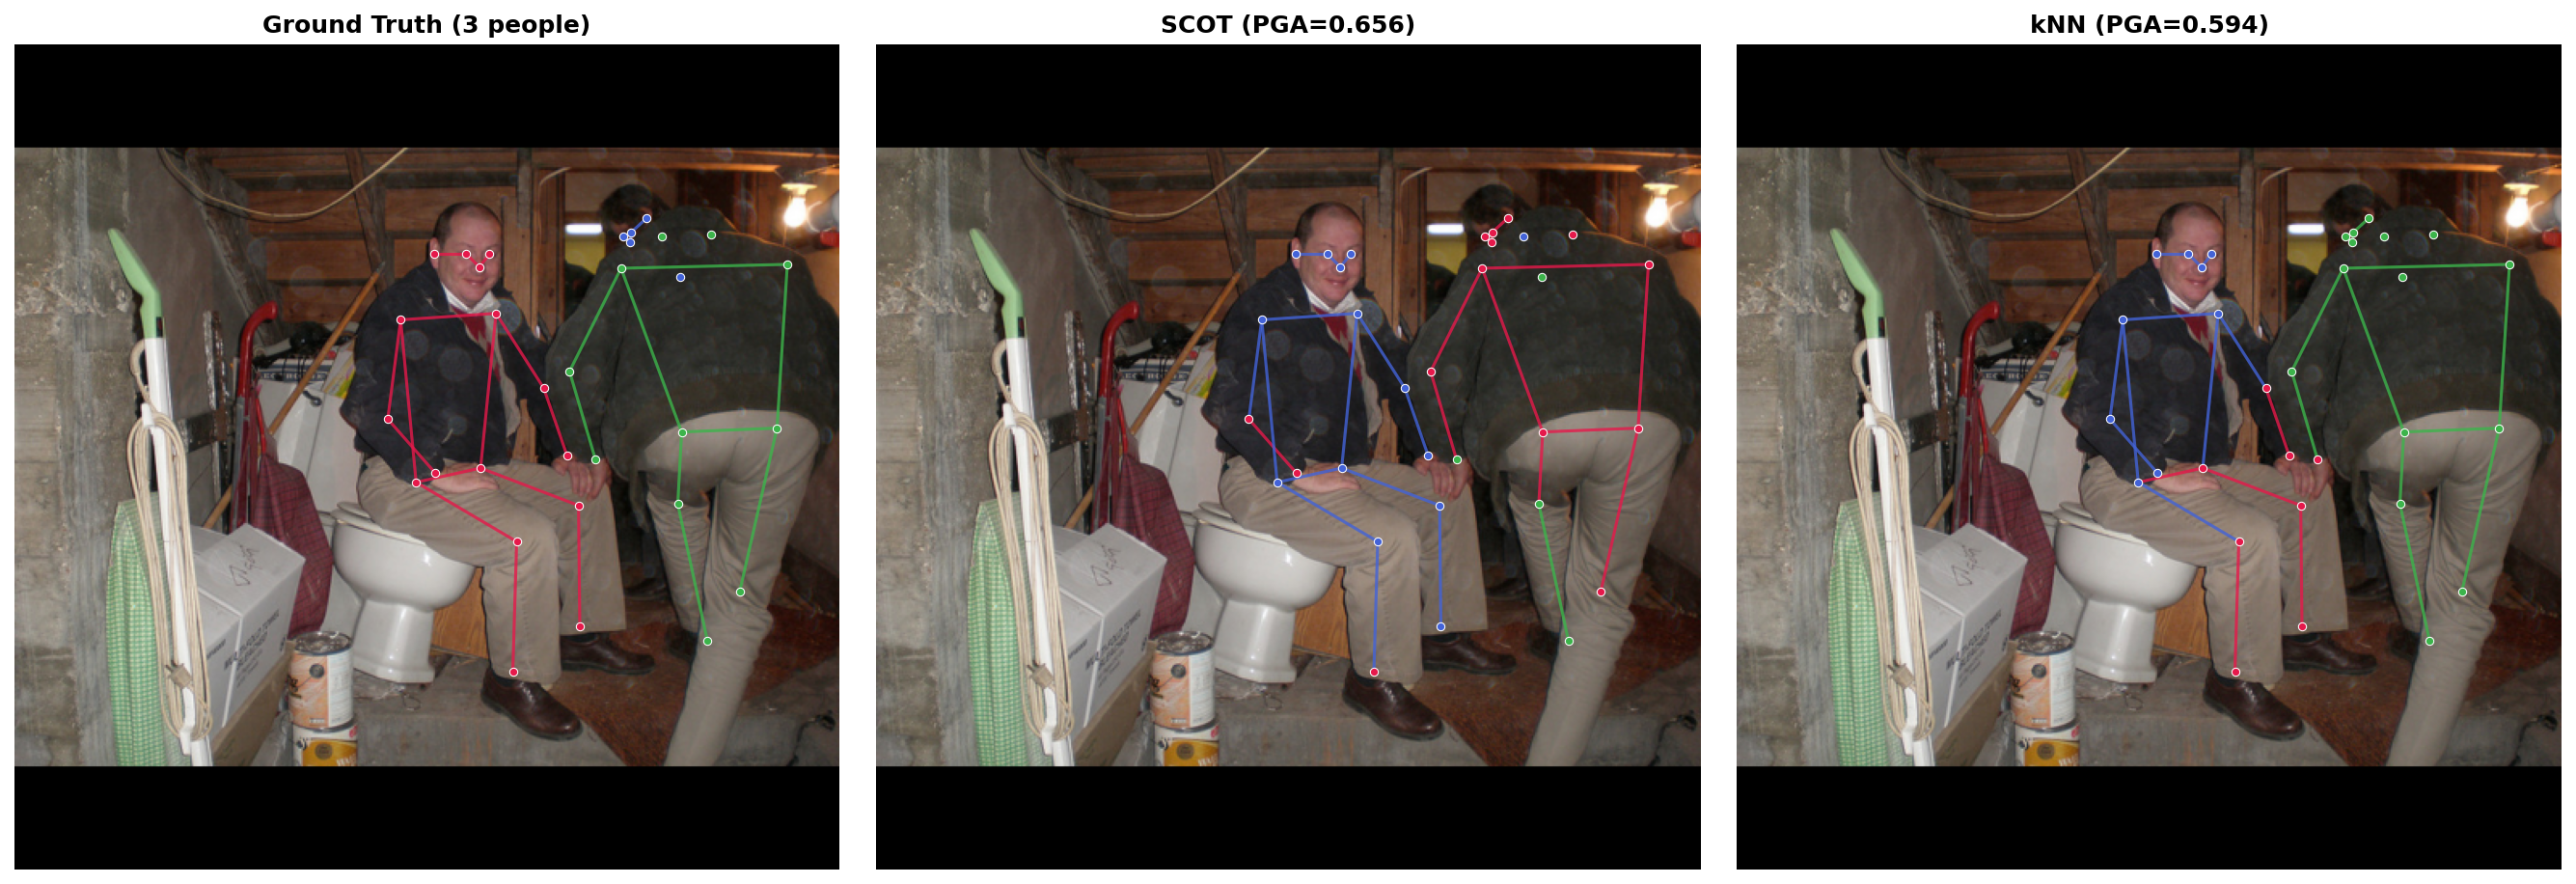
\includegraphics[width=\linewidth]{figures/demo_example_1.png}
  \caption{End-to-end demo on a COCO val2017 image with 3 heavily overlapping people. Left: ground truth person assignments. Centre: SCOT prediction (PGA=0.656). Right: kNN prediction (PGA=0.594). Skeleton edges are coloured by predicted person assignment.}
  \label{fig:demo_example_1}
\end{figure}

This is a hard scene --- three people seated close together with significant occlusion, exactly the scenario where pose grouping is most difficult. Neither method achieves high PGA, but SCOT outperforms kNN by 6.2 points (0.656 vs 0.594).

The failure mode for kNN is visible in the right panel: the seated person in the front and the person behind them are merged --- their body joints are mixed across the red and green clusters. kNN groups by embedding similarity, and when people overlap in 2D their embeddings are similar enough that k-means cannot separate them cleanly.

SCOT does better because the type constraint is active. The two overlapping people each have a left shoulder, left hip, left knee, etc. SCOT forces these same-type joints into different person slots --- it is structurally impossible for two left shoulders to be assigned to the same person. The blue person (seated front) is more coherent in the SCOT panel than in kNN.

This illustrates the core argument for SCOT over clustering-based approaches: in crowded scenes with spatially overlapping people, the skeleton type structure provides disambiguating signal that embedding similarity alone cannot. The type constraint does not help in easy scenes (well-separated people) or for joints where types are already distinct (face keypoints), but it provides a meaningful advantage in exactly the hard cases where pose grouping matters most.


\subsubsection{Experiment 12 --- SCOT with depth}

To complete the comparison, SCOT was trained with depth enabled (\texttt{use\_depth: true}). This uses the same GAT configuration as the original experiments from Experiments 1--2: node features are $[x, y, z, v]$ and kNN edges are built in 3D space. The question: does SCOT's type constraint add value when depth already makes the problem easy?

\paragraph{Synthetic results.}

\begin{table}[H]
\centering
\footnotesize
\begin{tabular}{lccccc}
\toprule
Method & PGA & Std & NMI & ARI & Det F1 \\
\midrule
kNN (contrastive GAT, depth) & 0.994 & 0.022 & 0.990 & 0.988 & 1.000 \\
SCOT head (depth) & 0.901 & 0.134 & 0.990 & 0.988 & 0.969 \\
\midrule
kNN (contrastive GAT, no depth) & 0.901 & 0.110 & 0.831 & 0.801 & 1.000 \\
SCOT head (no depth) & 0.923 & 0.105 & 0.803 & 0.767 & 0.997 \\
\bottomrule
\end{tabular}
\caption{SCOT with and without depth on synthetic test set.}
\end{table}

With depth, SCOT (0.901) does not beat kNN (0.994) --- a 9.3 point gap. This is the opposite of the no-depth result where SCOT beat kNN by 3.7 points. Depth makes the problem so easy for kNN that the embeddings are near-perfect (NMI 0.990) and k-means trivially recovers the correct groups. There are no type collisions to resolve because people are already well-separated in 3D. The type constraint cannot add value when the problem is already solved, and the Sinkhorn approximation is less precise than exact k-means on clean embeddings.

The training dynamics confirm this: the GAT loss drops to 0.002 (vs 0.050 without depth) and the head loss to 0.006 (vs 0.024). The model converges much faster but to a worse solution than kNN because the transport plan introduces noise that k-means does not have.

\paragraph{COCO transfer results.}

\begin{table}[H]
\centering
\footnotesize
\begin{tabular}{lccccc}
\toprule
Method & PGA & Std & NMI & ARI & Det F1 \\
\midrule
kNN (contrastive GAT, depth) & 0.839 & 0.194 & 0.758 & 0.696 & 1.000 \\
SCOT head (depth) & 0.812 & 0.210 & 0.758 & 0.696 & 0.982 \\
\midrule
kNN (contrastive GAT, no depth) & 0.879 & 0.170 & 0.837 & 0.782 & 1.000 \\
SCOT head (no depth) & 0.862 & 0.174 & 0.835 & 0.779 & 0.988 \\
\bottomrule
\end{tabular}
\caption{COCO val2017 results with and without depth.}
\end{table}

Per-joint accuracy on COCO with depth:

\begin{table}[H]
\centering
\footnotesize
\begin{tabular}{lccc}
\toprule
Joint & kNN (depth) & SCOT (depth) & SCOT (no depth) \\
\midrule
nose & 0.845 & 0.799 & 0.846 \\
left eye & 0.827 & 0.778 & 0.818 \\
right eye & 0.831 & 0.759 & 0.797 \\
left ear & 0.797 & 0.721 & 0.766 \\
right ear & 0.821 & 0.710 & 0.733 \\
left shoulder & 0.842 & 0.819 & 0.879 \\
right shoulder & 0.842 & 0.823 & 0.885 \\
left elbow & 0.835 & 0.792 & 0.830 \\
right elbow & 0.841 & 0.788 & 0.830 \\
left wrist & 0.839 & 0.776 & 0.804 \\
right wrist & 0.843 & 0.774 & 0.802 \\
left hip & 0.827 & 0.817 & 0.878 \\
right hip & 0.827 & 0.816 & 0.878 \\
left knee & 0.820 & 0.784 & 0.834 \\
right knee & 0.811 & 0.777 & 0.832 \\
left ankle & 0.764 & 0.742 & 0.794 \\
right ankle & 0.770 & 0.737 & 0.790 \\
\bottomrule
\end{tabular}
\caption{Per-joint accuracy on COCO. No-depth SCOT beats with-depth SCOT on every joint.}
\end{table}


\paragraph{Analysis.}

\textbf{1. Depth hurts SCOT on COCO even more than it hurts kNN.} SCOT drops from 0.862 (no depth) to 0.812 (with depth) on COCO --- a 5.0 point penalty. kNN's depth penalty is 4.0 points (0.879 $\to$ 0.839). The depth domain gap compounds with SCOT's existing transfer sensitivity because the Sinkhorn transport plan is more affected by noisy features than k-means.

\textbf{2. No-depth is strictly better for COCO transfer regardless of method.} The complete ranking on COCO:

\begin{table}[H]
\centering
\footnotesize
\begin{tabular}{lc}
\toprule
Method & COCO PGA \\
\midrule
kNN (no depth) & \textbf{0.879} \\
SCOT (no depth) & 0.862 \\
kNN (with depth) & 0.839 \\
SCOT (with depth) & 0.812 \\
\bottomrule
\end{tabular}
\caption{All methods ranked by COCO PGA.}
\end{table}

No-depth beats with-depth by $\sim$4--5 points across the board. This confirms the depth finding from Experiment~9: ground truth synthetic depth and MiDaS estimated depth are different enough that the model learns to rely on a signal that degrades at inference on real data.

\textbf{3. SCOT's advantage only exists when the problem is hard.} With depth, kNN at 0.994 leaves no room for improvement --- the type constraint is solving a problem that does not exist. Without depth, kNN drops to 0.901 and the type constraint provides genuine value (SCOT 0.923). This is the correct interpretation of SCOT: it is not a universally better grouping method, it is a method that adds value specifically when spatial proximity alone is insufficient to separate people.

\textbf{4. Per-joint accuracy confirms no-depth SCOT dominates across every joint.} No-depth SCOT beats with-depth SCOT on all 17 joints on COCO, with the largest gains on the joints where depth should theoretically help most: shoulders (+6.0/+6.2), hips (+6.1/+6.2), knees (+5.0/+5.5). The depth signal is so unreliable on COCO that even joints where 3D separation would be most informative are better served by a 2D-only model with hard type constraints.


\subsubsection{Experiment 13 --- Residual SCOT (spatial prior + learned correction)}

\paragraph{Motivation.}

SCOT beats kNN on synthetic data but loses on COCO. One hypothesis for why: kNN is a local, greedy method --- each keypoint independently picks its nearest cluster centre. On easy scenes where people are well-separated, greedy is optimal. OT is a global method --- it finds the best overall assignment considering all keypoints simultaneously. That global reasoning helps on hard scenes (overlapping people) but on easy scenes it introduces noise from the Sinkhorn entropy regularisation, which smears assignments that should be sharp.

The idea: decompose the cost matrix into a spatial prior and a learned correction:
\[
C_{\text{final}} = C_{\text{spatial}} + \lambda \cdot C_{\text{learned}}
\]

$C_{\text{spatial}}$ is the squared distance from each keypoint to $K$ spatial centroids computed via k-means on 2D positions (detached, not learned). This encodes geometric proximity --- equivalent to what kNN uses. $C_{\text{learned}}$ is the squared distance from encoded GAT embeddings to learned prototypes --- the same cost as vanilla SCOT.

On easy scenes, $C_{\text{spatial}}$ already has the right answer and the learned residual barely matters. On hard scenes, $C_{\text{spatial}}$ is ambiguous and $C_{\text{learned}}$ provides the discriminative correction. The spatial prior anchors easy cases, the learned cost handles hard cases.

This was implemented in a separate file (\texttt{ot\_head\_residual.py}) to preserve the original SCOT head for ablation. The $\lambda$ parameter was set to 0.2, meaning the spatial cost contributes 80\% and the learned cost 20\%.

\paragraph{Synthetic results.}

\begin{table}[H]
\centering
\footnotesize
\begin{tabular}{lccccc}
\toprule
Method & PGA & Std & NMI & ARI & Det F1 \\
\midrule
kNN (no depth) & 0.901 & 0.110 & 0.831 & 0.801 & 1.000 \\
kNN (Residual SCOT GAT) & 0.884 & 0.119 & 0.801 & 0.766 & 1.000 \\
SCOT (no depth) & 0.923 & 0.105 & 0.803 & 0.767 & 0.997 \\
Residual SCOT ($\lambda$=0.2) & 0.909 & 0.106 & 0.801 & 0.766 & 0.994 \\
\bottomrule
\end{tabular}
\caption{Residual SCOT vs vanilla SCOT on synthetic test set.}
\end{table}

Per-joint comparison on synthetic data:

\begin{table}[H]
\centering
\footnotesize
\begin{tabular}{lccc}
\toprule
Joint & kNN & SCOT & Residual SCOT \\
\midrule
nose & 0.888 & 0.895 & 0.872 \\
left eye & 0.889 & 0.907 & 0.891 \\
right eye & 0.891 & 0.878 & 0.885 \\
left ear & 0.905 & 0.902 & 0.875 \\
right ear & 0.900 & 0.915 & 0.896 \\
left shoulder & 0.924 & 0.950 & 0.942 \\
right shoulder & 0.911 & 0.950 & 0.953 \\
left elbow & 0.900 & 0.965 & 0.945 \\
right elbow & 0.899 & 0.931 & 0.923 \\
left wrist & 0.905 & 0.939 & 0.908 \\
right wrist & 0.864 & 0.891 & 0.893 \\
left hip & 0.889 & 0.968 & 0.919 \\
right hip & 0.886 & 0.944 & 0.932 \\
left knee & 0.872 & 0.947 & 0.921 \\
right knee & 0.886 & 0.919 & 0.920 \\
left ankle & 0.818 & 0.897 & 0.911 \\
right ankle & 0.805 & 0.896 & 0.870 \\
\bottomrule
\end{tabular}
\caption{Per-joint accuracy. Residual SCOT falls between kNN and SCOT on most joints.}
\end{table}

\paragraph{COCO transfer results.}

\begin{table}[H]
\centering
\footnotesize
\begin{tabular}{lcccc}
\toprule
Method & Synthetic & COCO & Transfer \\
\midrule
kNN (no depth) & 0.901 & 0.879 & $-2.2$ \\
SCOT (no depth) & 0.923 & 0.862 & $-6.1$ \\
Residual SCOT ($\lambda$=0.2) & 0.909 & 0.859 & $-5.0$ \\
\bottomrule
\end{tabular}
\caption{Transfer comparison. Residual SCOT's gap is slightly smaller but the difference is marginal.}
\end{table}

Full COCO results:

\begin{table}[H]
\centering
\footnotesize
\begin{tabular}{lccccc}
\toprule
Method & PGA & Std & NMI & ARI & Det F1 \\
\midrule
kNN (no depth) & 0.879 & 0.170 & 0.837 & 0.782 & 1.000 \\
SCOT (no depth) & 0.862 & 0.174 & 0.835 & 0.779 & 0.988 \\
Residual SCOT ($\lambda$=0.2) & 0.859 & 0.177 & 0.828 & 0.770 & 0.990 \\
\bottomrule
\end{tabular}
\caption{COCO val2017 results.}
\end{table}


\paragraph{Analysis.}

\textbf{1. Residual SCOT beats kNN but underperforms vanilla SCOT on synthetic data.} At 0.909, Residual SCOT is 2.5 points above kNN (0.884) but 1.4 points below SCOT (0.923). The spatial prior anchors assignments toward k-means centroids, which helps on easy scenes but constrains the learned cost from making the corrections that SCOT makes on hard scenes. The per-joint pattern confirms this --- SCOT gets 0.968 on left hip vs 0.919 for Residual SCOT, 0.965 on left elbow vs 0.945. The spatial prior is holding back the learned signal on exactly the joints where SCOT excels.

\textbf{2. On COCO the difference is negligible.} Residual SCOT (0.859) is within noise of SCOT (0.862). The transfer gap is slightly smaller ($-5.0$ vs $-6.1$), which was the hypothesis --- the spatial prior should be more robust to domain shift. But the improvement is marginal and not worth the added complexity (k-means centroid computation per forward pass, extra hyperparameter $\lambda$).

\textbf{3. The spatial prior doesn't help because it's redundant.} The k-means centroids computed from 2D positions encode the same information that the kNN graph edges already provide. The GAT has already absorbed spatial proximity through message passing --- the contrastive loss then separates the embeddings by person identity. Adding spatial centroids back into the cost matrix is giving the model information it already has, weighted against the learned signal that provides something new.

\textbf{4. Vanilla SCOT is the better formulation.} The learned cost from GAT embeddings is the right signal on its own. The spatial prior dilutes it without meaningful benefit on either synthetic or COCO data. This is a useful ablation result --- it confirms that SCOT's performance comes from the learned cost and hard type constraints, not from spatial proximity which kNN already captures optimally.
